% Options for packages loaded elsewhere
\PassOptionsToPackage{unicode}{hyperref}
\PassOptionsToPackage{hyphens}{url}
%
\documentclass[
]{book}
\usepackage{lmodern}
\usepackage{amssymb,amsmath}
\usepackage{ifxetex,ifluatex}
\ifnum 0\ifxetex 1\fi\ifluatex 1\fi=0 % if pdftex
  \usepackage[T1]{fontenc}
  \usepackage[utf8]{inputenc}
  \usepackage{textcomp} % provide euro and other symbols
\else % if luatex or xetex
  \usepackage{unicode-math}
  \defaultfontfeatures{Scale=MatchLowercase}
  \defaultfontfeatures[\rmfamily]{Ligatures=TeX,Scale=1}
\fi
% Use upquote if available, for straight quotes in verbatim environments
\IfFileExists{upquote.sty}{\usepackage{upquote}}{}
\IfFileExists{microtype.sty}{% use microtype if available
  \usepackage[]{microtype}
  \UseMicrotypeSet[protrusion]{basicmath} % disable protrusion for tt fonts
}{}
\makeatletter
\@ifundefined{KOMAClassName}{% if non-KOMA class
  \IfFileExists{parskip.sty}{%
    \usepackage{parskip}
  }{% else
    \setlength{\parindent}{0pt}
    \setlength{\parskip}{6pt plus 2pt minus 1pt}}
}{% if KOMA class
  \KOMAoptions{parskip=half}}
\makeatother
\usepackage{xcolor}
\IfFileExists{xurl.sty}{\usepackage{xurl}}{} % add URL line breaks if available
\IfFileExists{bookmark.sty}{\usepackage{bookmark}}{\usepackage{hyperref}}
\hypersetup{
  pdftitle={Testing for Measurement Invariance with Many Groups},
  pdfauthor={André Pirralha},
  hidelinks,
  pdfcreator={LaTeX via pandoc}}
\urlstyle{same} % disable monospaced font for URLs
\usepackage{longtable,booktabs}
% Correct order of tables after \paragraph or \subparagraph
\usepackage{etoolbox}
\makeatletter
\patchcmd\longtable{\par}{\if@noskipsec\mbox{}\fi\par}{}{}
\makeatother
% Allow footnotes in longtable head/foot
\IfFileExists{footnotehyper.sty}{\usepackage{footnotehyper}}{\usepackage{footnote}}
\makesavenoteenv{longtable}
\usepackage{graphicx,grffile}
\makeatletter
\def\maxwidth{\ifdim\Gin@nat@width>\linewidth\linewidth\else\Gin@nat@width\fi}
\def\maxheight{\ifdim\Gin@nat@height>\textheight\textheight\else\Gin@nat@height\fi}
\makeatother
% Scale images if necessary, so that they will not overflow the page
% margins by default, and it is still possible to overwrite the defaults
% using explicit options in \includegraphics[width, height, ...]{}
\setkeys{Gin}{width=\maxwidth,height=\maxheight,keepaspectratio}
% Set default figure placement to htbp
\makeatletter
\def\fps@figure{htbp}
\makeatother
\setlength{\emergencystretch}{3em} % prevent overfull lines
\providecommand{\tightlist}{%
  \setlength{\itemsep}{0pt}\setlength{\parskip}{0pt}}
\setcounter{secnumdepth}{5}
\usepackage{booktabs}
\usepackage{amsthm}
\makeatletter
\def\thm@space@setup{%
  \thm@preskip=8pt plus 2pt minus 4pt
  \thm@postskip=\thm@preskip
}
\makeatother
\usepackage[]{natbib}
\bibliographystyle{apalike}

\title{Testing for Measurement Invariance with Many Groups}
\author{\href{https://www.andrepirralha.com}{André Pirralha}}
\date{2020-10-15}

\begin{document}
\maketitle

{
\setcounter{tocdepth}{1}
\tableofcontents
}
\hypertarget{intro}{%
\chapter{Introduction}\label{intro}}

We have witnessed a surge of cross-national surveys over the past few years. Large international surveys, like the European Social Survey or the World Values Survey, provide researchers with unique opportunities to test their theories and hypothesis in diverse populations around the world. However, this availability of data is only very seldomly accompanied by the realization that the assumption of comparability of the survey instruments should not be given but tested instead. Before attributing any relevant differences between populations to substantial theoretical reasons, methodological and measurement causes should be explicitly ruled out by testing for measurement invariance. This workshop will introduce participants to the basics of measurement invariance testing with many groups. We will start by explaining what is measurement invariance and the major causes for measurement non-equivalence in surveys. Then we will proceed to discuss the three most common approaches to measurement invariance testing and end with a simple tutorial on how to test for measurement invariance with Multi-Group Confirmatory Factor Analysis (MG-CFA) using R environment.

\begin{quote}
This workshop is designed to be introductory and therefore I invite readers to follow the cited literature throughout this document and engage in further readings.
\end{quote}

\textbf{Workshop Content}

\begin{enumerate}
\def\labelenumi{\arabic{enumi}.}
\tightlist
\item
  \protect\hyperlink{intro}{Introduction}\\
\item
  \protect\hyperlink{comp}{Comparative Survey Research}
\item
  \protect\hyperlink{invariance}{Measurement Invariance}
\item
  \protect\hyperlink{check}{Checklist for Measurement Invariance with MG-CFA}
\item
  \protect\hyperlink{lavaan}{Testing for measurement invariance with lavaan in R}
\item
  \protect\hyperlink{home}{Take-Home Message}
\item
  \protect\hyperlink{further}{Further Reading}
\item
  \protect\hyperlink{ref}{References}
\end{enumerate}

\hypertarget{work-in-progress}{%
\section{Work in Progress}\label{work-in-progress}}

This document is also a work in progress. New versions with more resources and information should be completed soon. Check my website to keep up with the progress \href{https://andrepirralha.com}{www.andrepirralha.com}

\hypertarget{comp}{%
\chapter{Comparative survey research}\label{comp}}

Cross-national and cross-cultural comparative surveys are a very important resource for the Social Sciences. According to the \href{https://www.gesis.org/angebot/daten-analysieren/weitere-sekundaerdaten/uebersichten/overview-of-comparative-surveys-worldwide}{Overview of Comparative Surveys Worldwide}, more than 90 cross-national comparative surveys have been conducted around the world since 1948.

Even though surveys can aim to fulfill different purposes, generally they aim to estimate population means, totals or distributions or relationships between variables. A comparative survey will aim to compare these levels or relationships across groups (national or otherwise).

\textbackslash begin\{figure\}
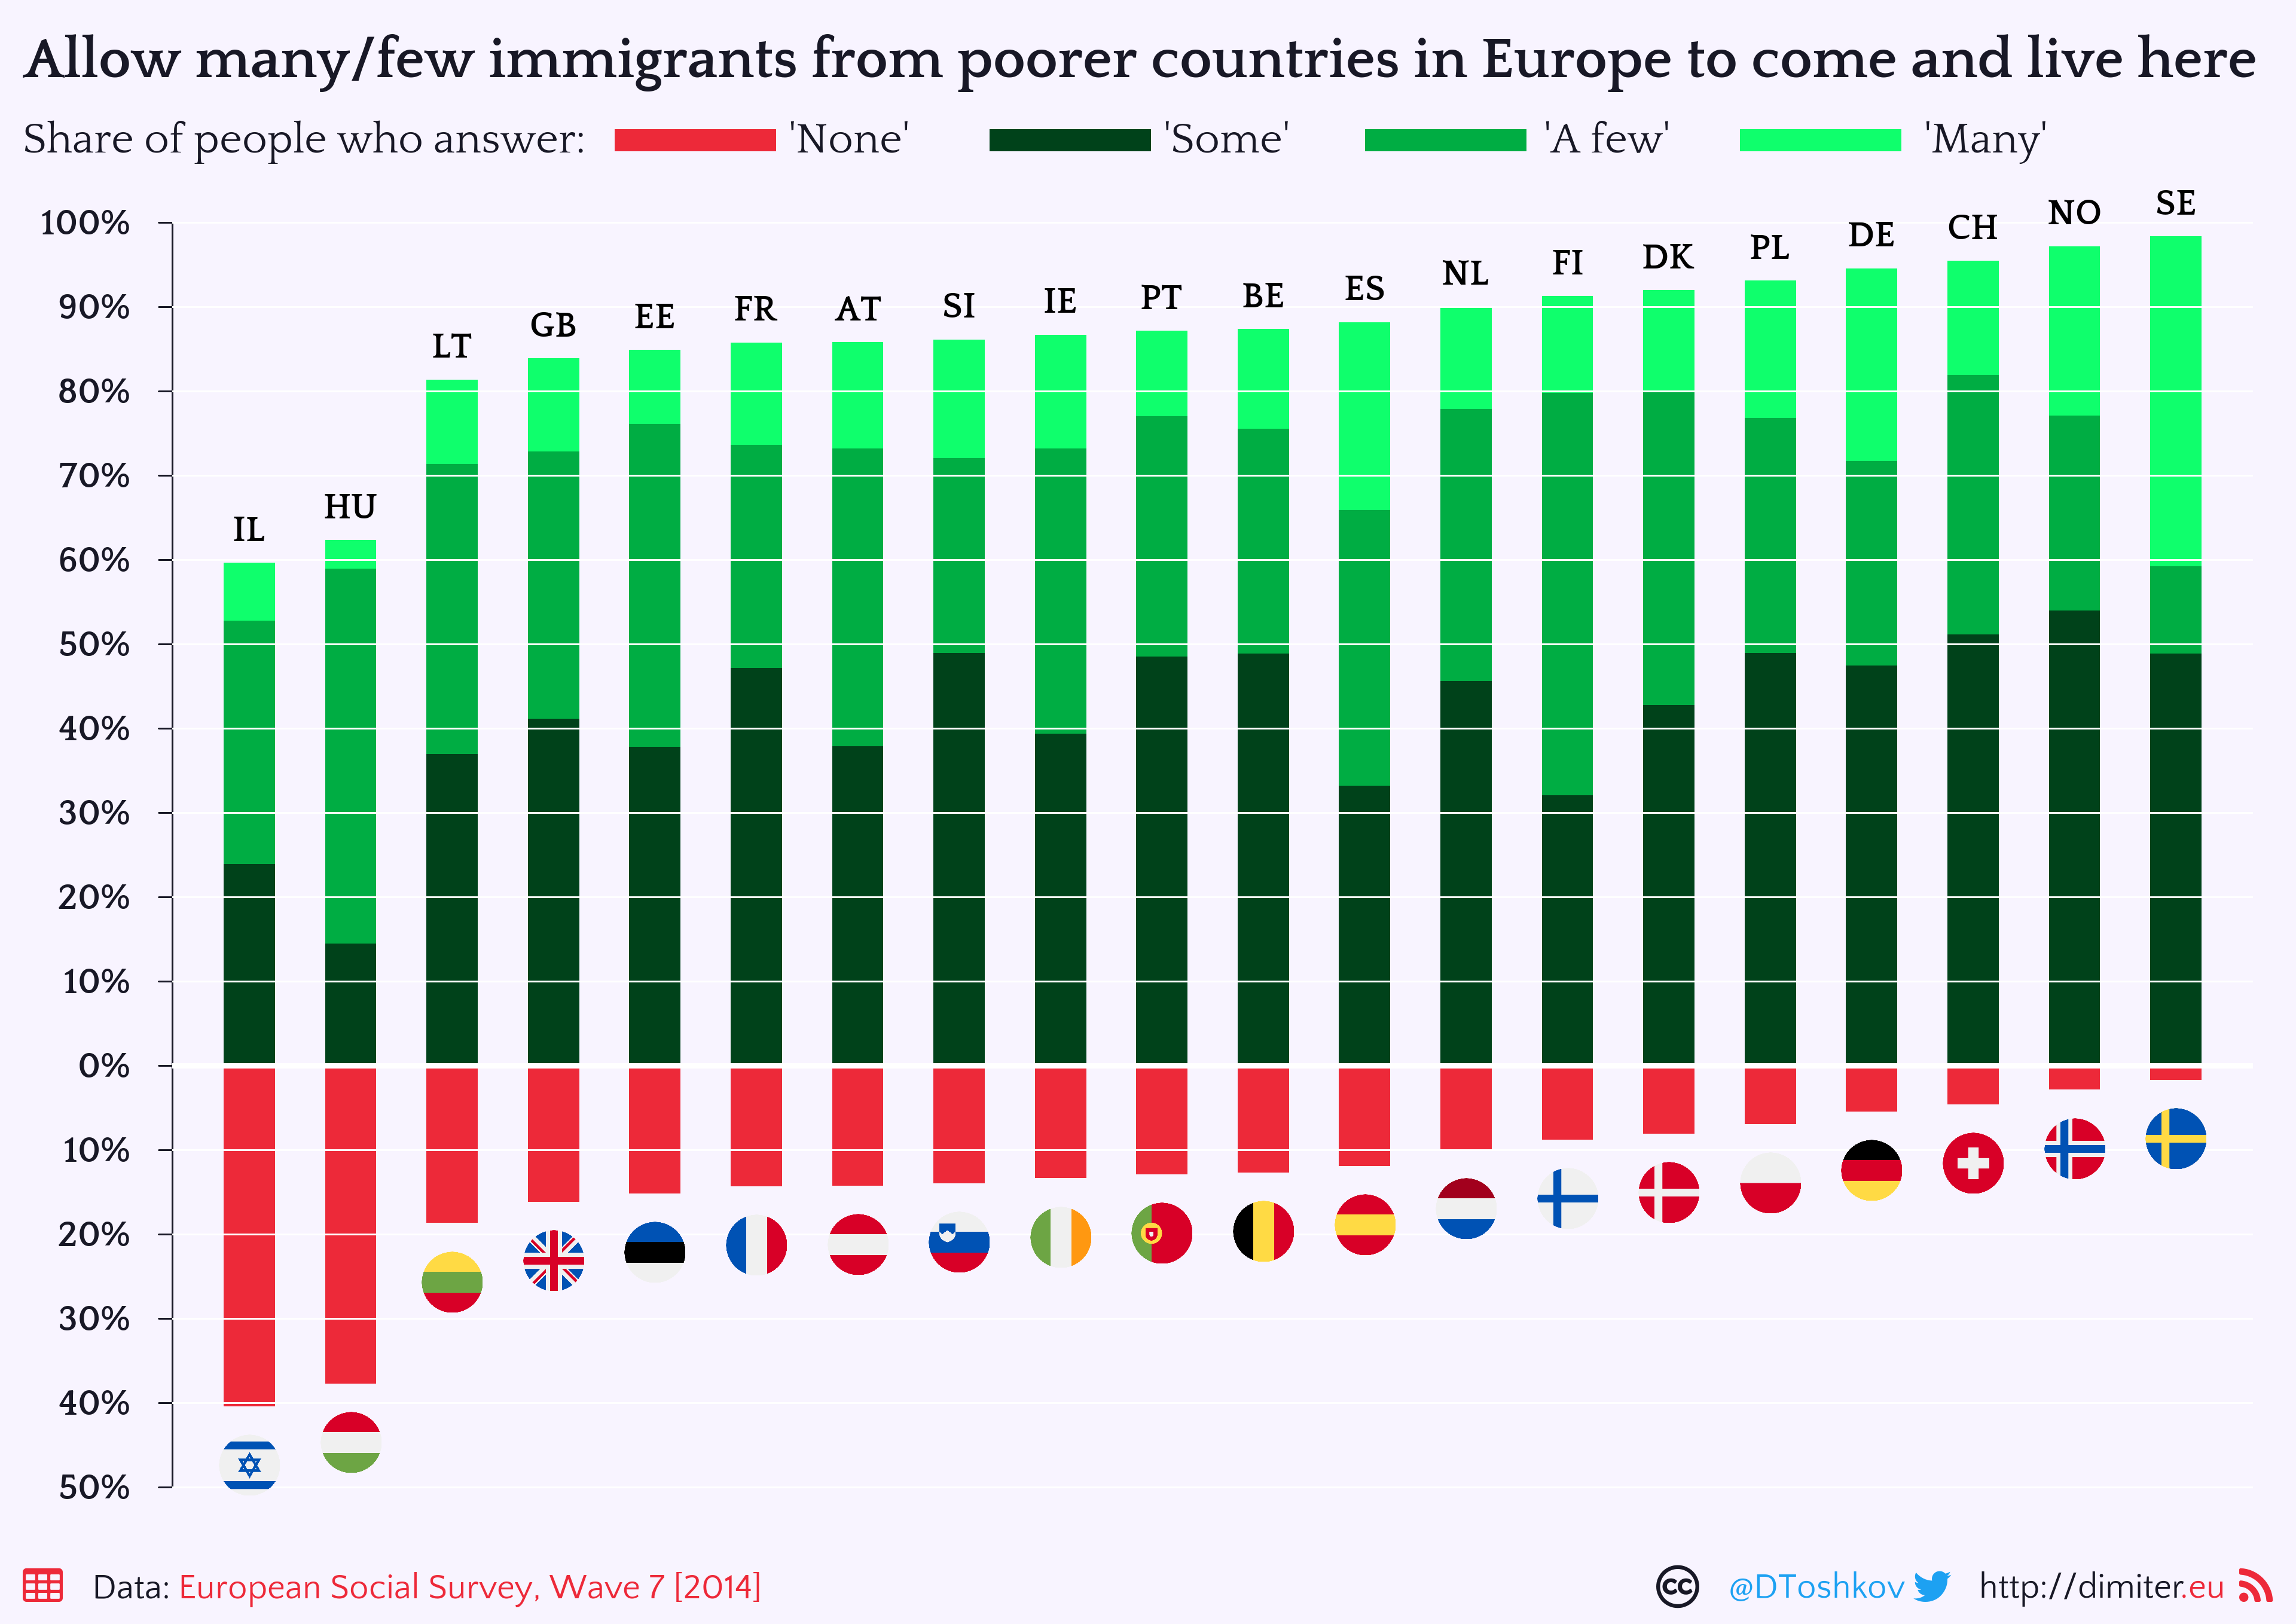
\includegraphics[width=0.8\linewidth]{bar_graph} \textbackslash caption\{Comparative percentages by country regarding immigration tolerance, from the European Social Survey Round 7. Source: \href{https://dimiter.eu/Visualizations_files/ESS/Visualizing_ESS_data.html\#saving_the_visualization}{Dimiter Toshkov 2020}\}\label{fig:bar}
\textbackslash end\{figure\}

Figure 2.1 shows a rather common application of a comparative survey. The groups, in this case European countries, are compared on their percentage shares on the answer to the question about allowing more immigrants.

However, what we see in this graph is only the final abstraction of very long process that typically surveys, and most particularly cross-national surveys, must go through. This process is sometimes called survey lifecycle and goes from design to dissemination.

\begin{figure}
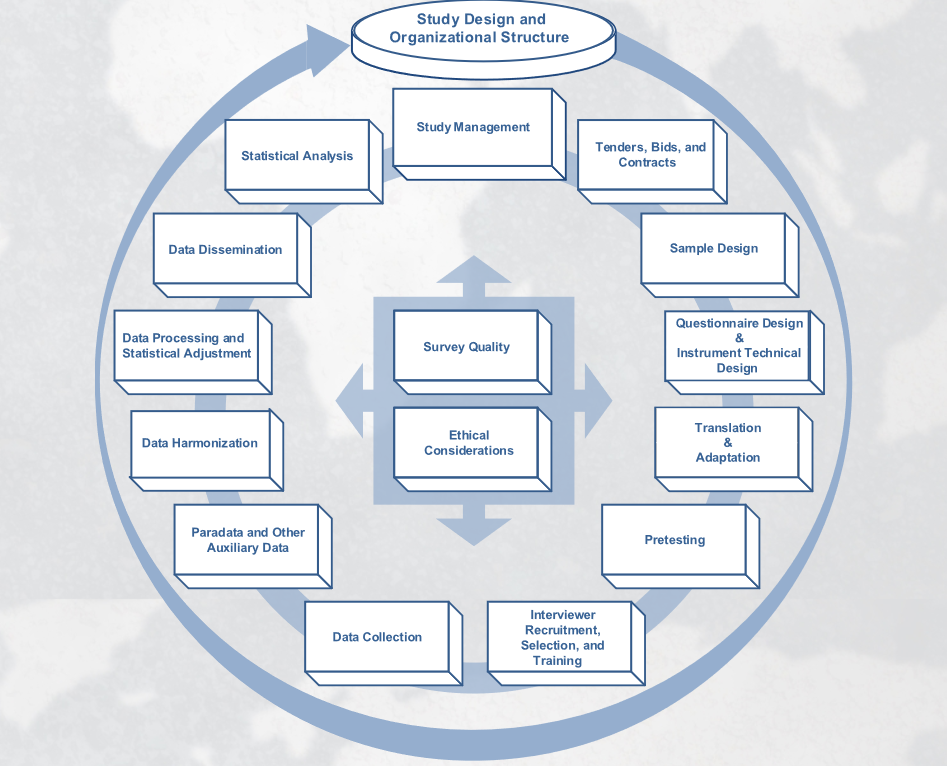
\includegraphics[width=0.8\linewidth]{lifecycle} \caption{Survey Lifecycle. Source: [Cross Cultural Survey Guidelines](https://ccsg.isr.umich.edu/chapters)}\label{fig:cycle}
\end{figure}

\hypertarget{survey-error}{%
\section{Survey Error}\label{survey-error}}

\begin{quote}
\emph{Survey error is any error arising from the survey process that contributed to the deviation of an estimate from its true parameter values.} \citep{Biemer}
\end{quote}

But regardless of how much we can try to prevent it, survey errors in one form or another will always occur. And survey errors might affect the estimates and their comparability.

This applies both to when we compare data from different surveys and comparisons of sub-groups within the same survey.

The comparability of survey measurements is an issue that should be thoughtfully considered before drawing substantive conclusions from comparative surveys.

\begin{figure}
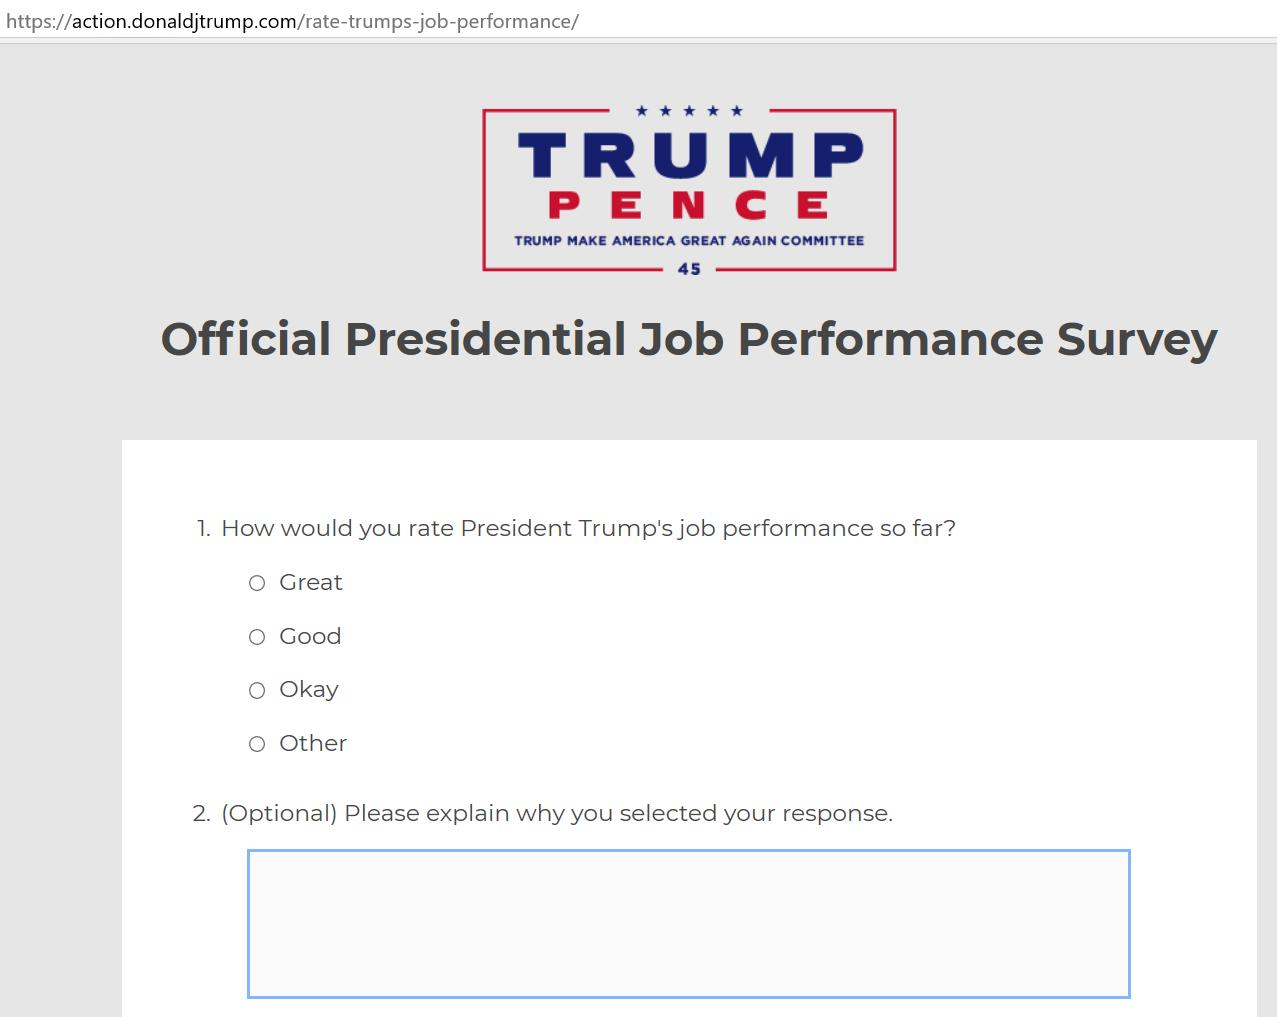
\includegraphics[width=0.8\linewidth]{trump_pence} \caption{Slighty problematic survey question. Source: [badsurveyq](https://twitter.com/badsurveyq)}\label{fig:trump}
\end{figure}

Survey error can be classified in two components:

\begin{quote}
Random error is caused by any factors that randomly affect measurement of the variable
\end{quote}

\begin{quote}
Systematic error is caused by any factors that systematically affect measurement of the variable
\end{quote}

Survey group comparability problems come from systematic error or ``Bias''\footnote{systematic error and ``Bias'' are terms used interchangeably in the literature and they refer to deviations that are not due to chance alone.}.

What is particular about comparative surveys is that there are at least two different survey statistics. Therefore, each one of these statistics is subject to different sources of error. If the overall statistics are differently affected by the error, this will cause some form of ``bias'' in the comparison.

\begin{quote}
In other words, besides substantive differences between survey statistics, there might be systematic differences caused by survey error.
\end{quote}

\hypertarget{total-survey-error-framework}{%
\section{Total Survey Error framework}\label{total-survey-error-framework}}

\begin{quote}
Total survey error is the accumulation of all errors that may arise in the design, collection, processing and analysis of survey data.
\end{quote}

The Total Survey Error offers an elegant framework to describe survey errors and the several sources of error that are rooted within the survey lifecycle.

\begin{figure}
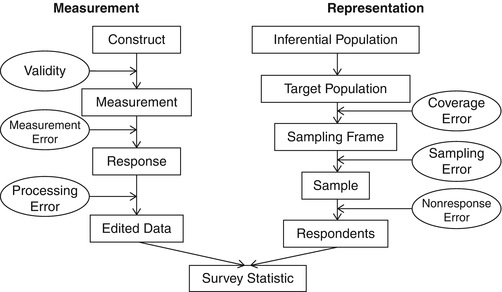
\includegraphics[width=0.8\linewidth]{total_survey_error} \caption{Source: @Groves2010}\label{fig:ext}
\end{figure}

As it can be seen in figure 2.4, there is a ``representation'' and a ``measurement'' side.

Systematic representation errors include:

\begin{itemize}
\tightlist
\item
  coverage error
\item
  sampling error
\item
  nonresponse
\end{itemize}

Systematic error in measurement include:

\begin{itemize}
\tightlist
\item
  validity
\item
  processing
\item
  measurement error
\end{itemize}

Measurement error includes: response error, interviewer-induced response effects, social desirability, methods effects, response styles.

\begin{quote}
Here we will focus on the Measurement side
\end{quote}

\hypertarget{the-bias-framework}{%
\section{The ``Bias'' framework}\label{the-bias-framework}}

The TSE error classification is analogous to the \textbf{``Bias''} framework in the field of cross-cultural psychology. Under this framework, \citet{VandeVijver1997} distinguished between ``construct'', ``item'', and ``method'' bias which are essencially similar to the TSE's validity, measurement error and all the remaining errors.

\begin{quote}
The bias framework is developed from the perspective of cross-cultural psychology and attempts to provide a comprehensive taxonomy of all systematic sources of error that can challenge the inferences drawn from cross-cultural studies \citep{VandeVijver1997, VandeVijver2000, VandeVijver1997a, VandeVijver2004}.
\end{quote}

\hypertarget{construct-bias}{%
\subsection{Construct Bias}\label{construct-bias}}

Construct bias is present if the underlying construct measured is not the same across cultures.

\begin{itemize}
\tightlist
\item
  It can occur if a construct is differently defined or only has a partial overlap across cultural groups.
\end{itemize}

Example:

\begin{quote}
Varying definitions of happiness in Western and East Asian cultures \citep{Uchida2004}. In Western cultures, happiness tends to be defined in terms of individual achievement, whereas in East Asian cultures happiness is defined in terms of interpersonal connectedness.
\end{quote}

\hypertarget{method-bias}{%
\subsection{Method Bias}\label{method-bias}}

\begin{itemize}
\item
  Sample Bias: is the incomparability of samples due to cross-cultural variations in characteristics, such as different educational levels, students versus the general population, and urban versus rural residents
\item
  Instrument bias: involves systematic errors derived from instrument characteristics such as self-report bias in Likert-type scale measures. The systematic tendency of respondents to endorse certain response options on some basis other than the target construct (i.e., response styles) may affect the validity of cross- cultural comparisons \citep{VanHerk2004}.
\item
  Administration Bias: stems from administration conditions (e.g., data collection modes, group versus individual assessment), ambiguous instructions, interaction between administrators and respondents (e.g., halo effects), and communication problems (e.g., language differences, taboo topic).
\end{itemize}

\hypertarget{item-bias}{%
\subsection{Item Bias}\label{item-bias}}

\begin{itemize}
\item
  Occurs when an item has a different meaning across cultures. An item of a scale is biased if persons with the same target trait level, but coming from different cultures, are not equally likely to endorse the item (\citet{VandeVijver1997}; \citet{VandeVijver2013}).
\item
  Item bias can arise from poor translation, inapplicability of item contents in different cultures, or from items that trigger additional traits or have words with ambiguous connotations.
\end{itemize}

\hypertarget{preventing-survey-comparability-problems}{%
\section{Preventing survey comparability problems}\label{preventing-survey-comparability-problems}}

Following the TSE framework, the best way to reduce eventual comparability issues in survey data is to reduce the survey error to the very minimum and assuring that the persistent errors are most likely similar across the groups.

There is a vast literature discussing how to reduce TSE. However, two issues are particularly relevant to cross-cultural/national surveys.

\hypertarget{translation}{%
\subsection{Translation}\label{translation}}

TRAPD - Translation, Review, Adjudication, Pretesting, and Documentation

This method was proposed by \citet{Harkness2003}

Team approach to survey translation:

\begin{quote}
\begin{itemize}
\tightlist
\item
  \textbf{T}ranslators produce, independently from each other, initial translations
\end{itemize}
\end{quote}

\begin{quote}
\begin{itemize}
\tightlist
\item
  \textbf{R}eviewers review translations with the translators
\end{itemize}
\end{quote}

\begin{quote}
\begin{itemize}
\tightlist
\item
  \textbf{A}djudicator (one or more) decides whether the translation is ready
\end{itemize}
\end{quote}

\begin{quote}
\begin{itemize}
\tightlist
\item
  \textbf{P}retesting is the next step before going out to the field
\end{itemize}
\end{quote}

\begin{quote}
\begin{itemize}
\tightlist
\item
  \textbf{D}ocumentation should be constant during the entire process
\end{itemize}
\end{quote}

\hypertarget{question-coding-system-sqp}{%
\subsection{Question coding system: SQP}\label{question-coding-system-sqp}}

It offers an additional way to check question comparability by taking into account the different characteristics of the questions in the original and adapted versions.

\begin{quote}
\url{https://sqp.upf.edu/}
\end{quote}

\hypertarget{invariance}{%
\chapter{Measurement Invariance}\label{invariance}}

Measurement invariance addresses some of the statistical implications of the TSE and ``Bias'' frameworks and defines conditions that have to be fulfilled before inferences can be drawn about comparative conclusions dealing with constructs or scores in cross-national/cultural studies.

\begin{itemize}
\item
  Comparisons can only be made if the people in the different countries/cultures react similarly to the questions asked.
\item
  The measures should be ``functionally equivalent'' and the response models should be invariant across countries
\end{itemize}

\hypertarget{what-it-measurement-invariance}{%
\section{What it Measurement Invariance?}\label{what-it-measurement-invariance}}

Formal definition of invariance:

\begin{quote}
``whether or not, under different conditions of observing and studying phenomena, measurement operations yield measures of the same attribute'' \citep[p.~117]{Horn1992}.
\end{quote}

What implies?

\begin{quote}
Measurement invariance implies that using the same questionnaire in different groups (such as countries or at various points in time, or under different conditions) does measure the same construct in the same way \citep{Chen2008, Davidov2014, Horn1992, Millsap2011}.
\end{quote}

\hypertarget{how-to-test-for-it}{%
\section{How to test for it?}\label{how-to-test-for-it}}

The most common method to test measurement invariance is Multi-Group Confirmatory Factor Analysis (MGCFA).

\hypertarget{confirmatory-factor-analysis}{%
\subsection{Confirmatory Factor Analysis}\label{confirmatory-factor-analysis}}

CFA focuses on modeling the relationship between manifest (i.e., observed) indicators and underlying latent variables (factors). CFA is a special case of structural equation modeling (SEM) in which relationships among latent variables are modeled as covariances/correlations rather than as structural relationships (i.e., regressions). CFA can also be distinguished from exploratory factor analysis (EFA) in that CFA requires researchers to explicitly specify all characteristics of the hypothesized measurement model (e.g., the number of factors, pattern of indicator- factor relationships) to be examined whereas EFA is more data-driven.

\begin{figure}
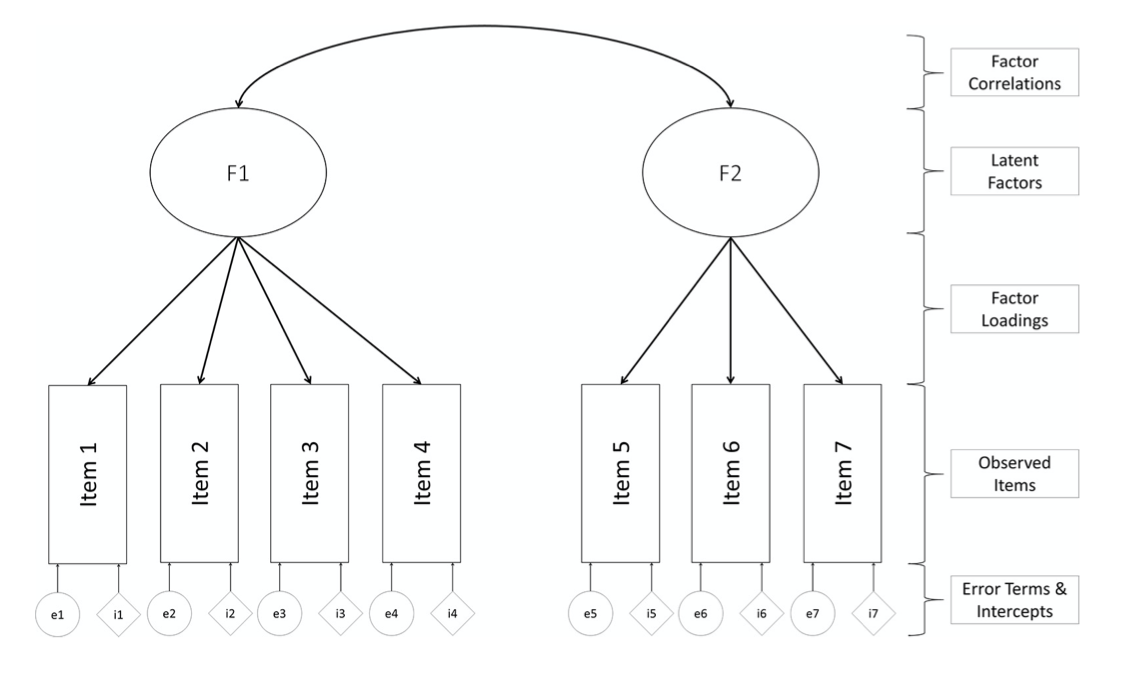
\includegraphics[width=0.8\linewidth]{confactor} \caption{Source: Wicherts & Dolan, 2010}\label{fig:cfa}
\end{figure}

For more information about confirmatory factor analysis see \citet{Brown2015}.

\hypertarget{multi-group-confirmatory-factor-analysis---mgcfa}{%
\subsection{Multi-Group Confirmatory Factor Analysis - MGCFA}\label{multi-group-confirmatory-factor-analysis---mgcfa}}

\begin{itemize}
\item
  With a single model tests whether a theoretical model fits several groups simultaneously
\item
  How? Because we constrain parameters to be equal across groups
\item
  MGCFA invariance testing model in practice is testing an hypothesis of whether a given theoretical model fits well to the data across the groups.
\item
  Depending on what parameters we constraint to be equal across groups, we test one or another level of invariance
\end{itemize}

\begin{figure}
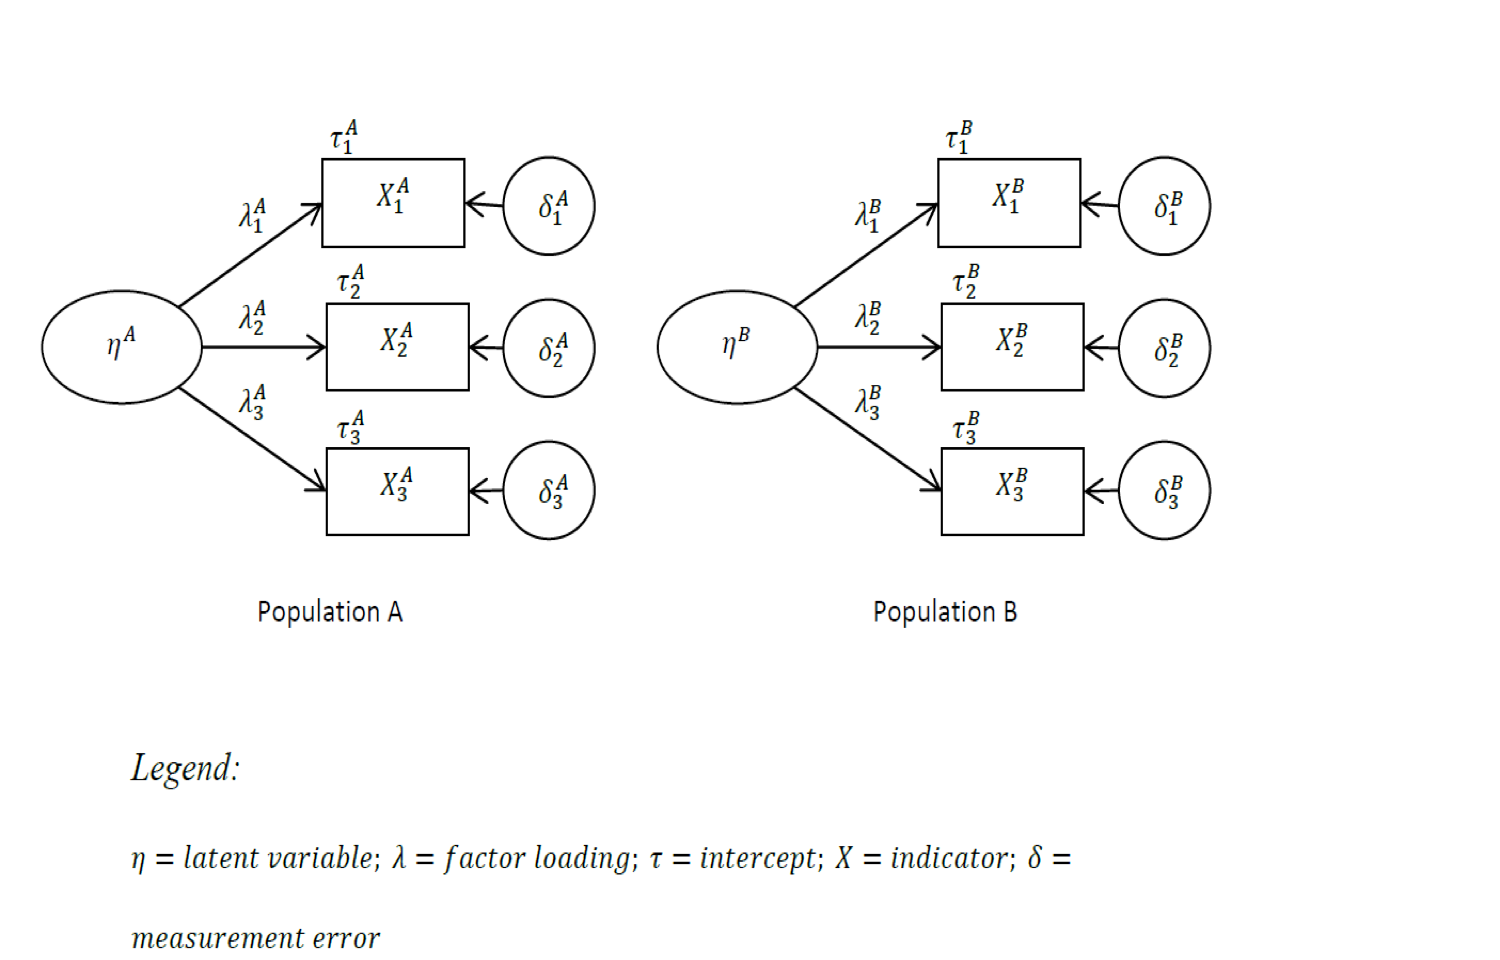
\includegraphics[width=0.8\linewidth]{multi_group} \caption{Source: Wicherts & Dolan, 2010}\label{fig:mgcfa}
\end{figure}

\hypertarget{invariance-testing-levels}{%
\section{Invariance Testing Levels}\label{invariance-testing-levels}}

Most research focus on 3 levels of measurement invariance:

\begin{enumerate}
\def\labelenumi{\arabic{enumi}.}
\item
  Configural Invariance (structural equivalence): the same model holds for all the groups
\item
  Metric Invariance (measurement unit equivalence): factor loadings (slopes) are the same across the groups
\end{enumerate}

\begin{quote}
Implication: The scale intervals are the same across groups because the loadings are the same in each group. When checked, allows comparing unstandardized regression coefficients and/or covariances across groups.
\end{quote}

\begin{enumerate}
\def\labelenumi{\arabic{enumi}.}
\setcounter{enumi}{2}
\tightlist
\item
  Scalar Invariance (Full score equivalence): the intercepts are the same across all countries being compared.
\end{enumerate}

\begin{quote}
Implication: Latent means can be compared across groups meaningfully.
\end{quote}

Following a bottom-up approach, each level is tested by setting cross-group constraints on parameters (loadings and intercepts) and comparing hierarchically more constrained models with less constrained ones.

At the configural level, loadings and intercepts are freely estimated.

At the metric level, loadings are constrained to be equal across groups and the intercepts are freely estimated.

The scalar invariance model is the most constrained, with both loadings and intercepts constrained to be equal across groups.

\hypertarget{response-function}{%
\subsection{Response Function}\label{response-function}}

The process by which a respondent arrives at an answer, that is the relationship between the respondent's ``opinion'' and the final answer, is called the response function. Figure 3.3 illustrates a possible response function

\begin{figure}

\includegraphics[width=0.8\linewidth]{response_function} \caption{Illustration of a Response Function. Source: Adapted from Wicherts & Dolan}\label{fig:response}
\end{figure}

The \emph{X} axis represents the latent variable mean; the \emph{Y} axis represents the response to a survey question item measuring the latent variable. The diagonal represents the functional relation between the latent variable and the (unstandardized) response to the survey question item in group G1.

\begin{quote}
Another way to thing about invariance testing is as a procedure to check whether the response functions across different groups are similar and can therefore be compared.
\end{quote}

\hypertarget{example}{%
\subsubsection{Example}\label{example}}

Let's imagine we have two groups. These groups are respondents answering the same survey questions in two different countries: Group 1 and Group 2.

\begin{figure}
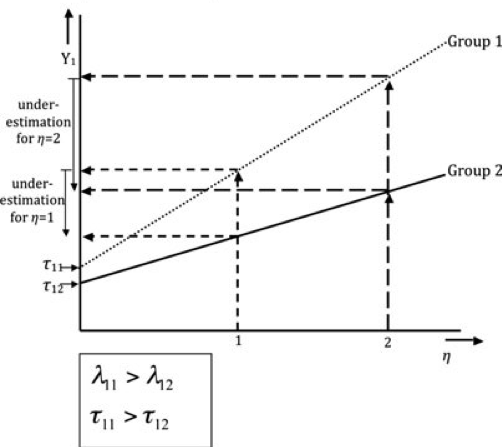
\includegraphics[width=0.8\linewidth]{Picture2} \caption{Source: Wicherts & Dolan, 2010}\label{fig:non}
\end{figure}

Figure 3.4 describes a configural invariance scenario. Both the factor loadings and intercepts are different across the groups, as is made clear by the different slopes and Y axis intersections for G1 and G2. Therefore, metric and scalar invariance do not hold in these groups and shouldn't be compared.

\begin{figure}
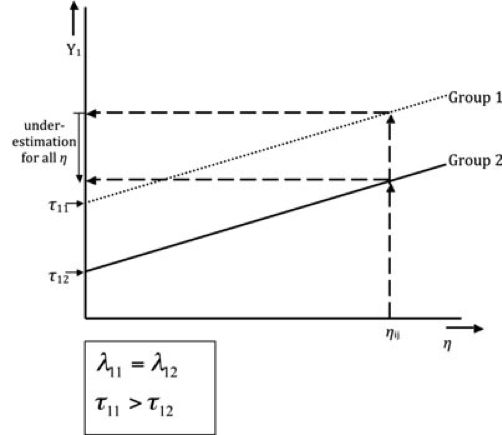
\includegraphics[width=0.8\linewidth]{Picture1} \caption{Source: Wicherts & Dolan, 2010}\label{fig:metric}
\end{figure}

Figure 3.5 describes metric invariance and scalar \textbf{non}invariance. The slopes are identical and therefore we can assume the factor loadings are the same across the groups.

\begin{figure}

\includegraphics[width=0.8\linewidth]{metric_scalar} \caption{Source: Wicherts & Dolan, 2010}\label{fig:metandscalar}
\end{figure}

Finally, figure 3.6 shows that the loadings are the same across the groups (similar slopes) and that the intercepts are approximately also the same.

\hypertarget{how-to-handle-noninvariance}{%
\section{How to handle Noninvariance}\label{how-to-handle-noninvariance}}

It is not uncommon to have noninvariance across groups. The literature shows several examples of scales that fail to be comparable across groups. Some examples:

\begin{quote}
\citet{Aleman2016} and \citet{SOKOLOV2018} recently showed that the Inglehart value scales are not comparable across all countries (but see \citet{Welzel2016}); \citet{Ariely2011} found that public support for democracy cannot be compared across countries in the World Value Survey (WVS); \citet{Lomazzi2017} demonstrated that gender-role attitudes are not comparable across all WVS countries; \citet{Davidov2008} showed that means of human values in the ESS may not be compared across all countries; \citet{Rudnev2018} found that the means of Seeman's alienation scale are not comparable cross-nationally.
\end{quote}

Several theoretical and more technical procedures have been discussed to overcome a potential noninvariant result.

Figure 3.7 compiles a great part of this discussion and can be used as a decision tree when necessary.

\begin{figure}
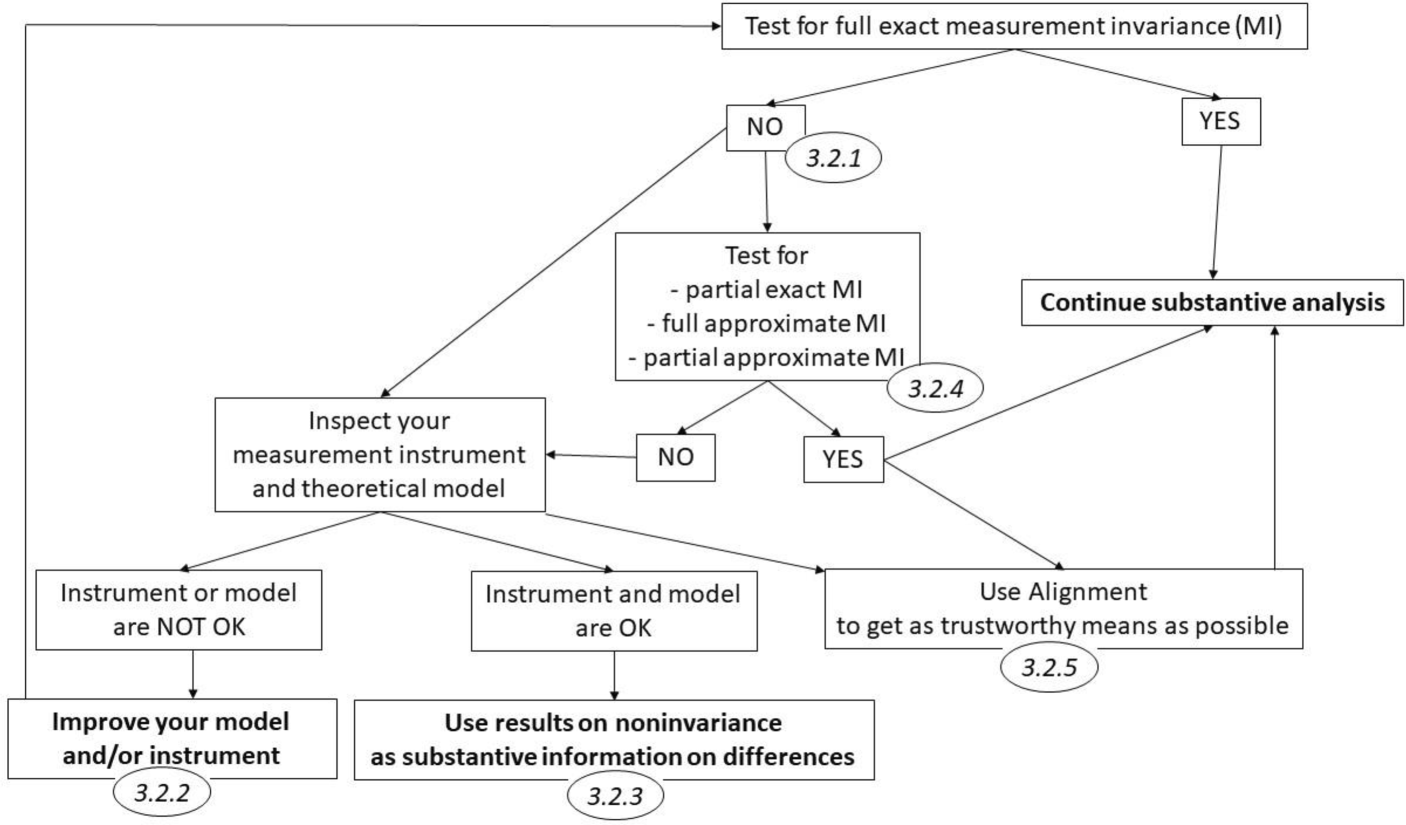
\includegraphics[width=0.8\linewidth]{decision_tree} \caption{Source: Wicherts & Dolan, 2010}\label{fig:tree}
\end{figure}

\hypertarget{partial-invariance-testing}{%
\subsection{Partial Invariance Testing}\label{partial-invariance-testing}}

Some authors consider that partial invariance is enough of a requisite for comparisons across groups to be made \citep{Byrne1989a, Steenkamp1998}.

Partial invariance is established when the parameters of at least two indicators are equal across groups.

This means to identify those items that are very different across groups and release them while making sure that at least two items per latent concept have equal loadings and intercepts.

While this approach has been frequently used, there are also some critics that see it as not enough to assure meaningful comparisons \citep{DeBeuckelaer2011, Steinmetz2018EstimationAC}.

\hypertarget{alternative-measurement-invariance-testing-procedures}{%
\subsection{Alternative Measurement Invariance Testing procedures}\label{alternative-measurement-invariance-testing-procedures}}

\hypertarget{exact-invariance-testing-alternative-approaches-to-mgcfa}{%
\subsubsection{Exact Invariance testing alternative approaches to MGCFA}\label{exact-invariance-testing-alternative-approaches-to-mgcfa}}

Multi-indicator Multiple Cause (MIMIC)

\begin{itemize}
\tightlist
\item
  MIMIC model permits both categorical and continuous individual difference variables (e.g., sex and age) but permits only a subset of the model parameters to vary as a function of these characteristic
\end{itemize}

See \citep{Kim2012}

Item Response Theory (IRT) Differential Item Functioning

\begin{itemize}
\tightlist
\item
  Aimed to categorical data
\end{itemize}

See \citep{Tay2015}

\begin{center}\rule{0.5\linewidth}{0.5pt}\end{center}

\hypertarget{approximate-invariance-a-conceptually-different-approach}{%
\subsubsection{Approximate Invariance: a conceptually different approach}\label{approximate-invariance-a-conceptually-different-approach}}

It is argued that a general measurement model using a CFA applies overly restrictive assumptions
that represent a theory-driven model \citep{Brown2015, Marsh2013}. Assumptions include that each measure loads on only one factor (e.g., assuming the absence of cross-loadings and residual correlations), the absence of effects from covariates, and the assumption of an exact invariant of the measures in MGCFA.

\begin{itemize}
\tightlist
\item
  In analysis of cross-national data, equality constraints tend to lead to the rejection of the tested model and often produce poor model fit statistics. Increasing the methodological sophistication and availability of statistical tools provide ways of quantifying uncertainty in the hypothesis through the estimation of possible values in the population rather than depending on only a single value for many populations.
\end{itemize}

\begin{figure}
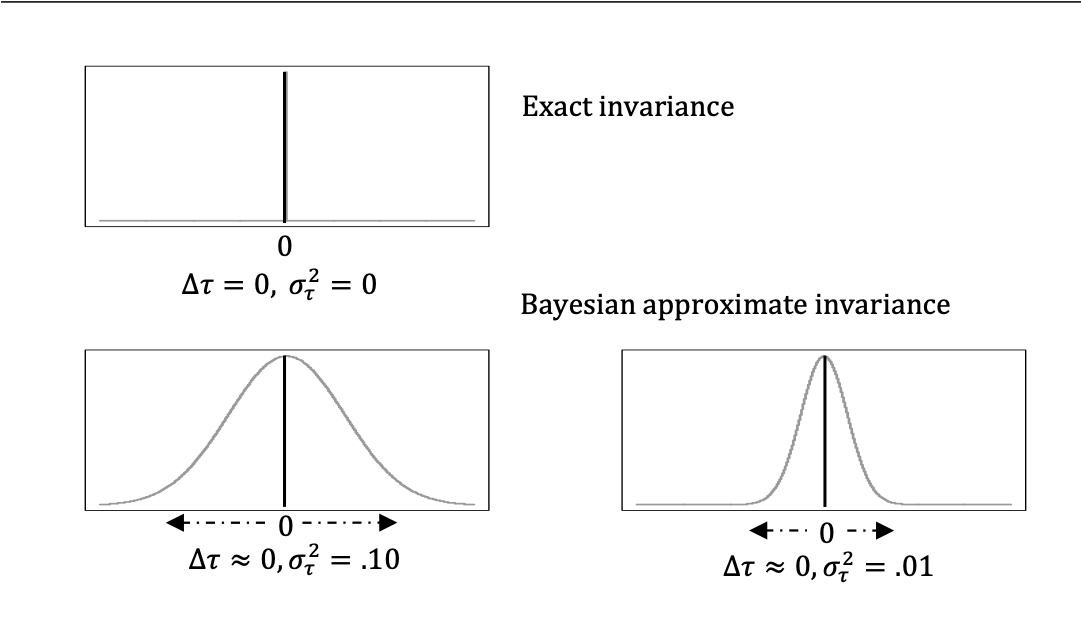
\includegraphics[width=0.8\linewidth]{approximate} \caption{Source: Wicherts & Dolan, 2010}\label{fig:approximate}
\end{figure}

Source \citep{Desa2018}

Approximate Invariance techniques:

\begin{itemize}
\item
  Alignment invariance \citep{Muthen2018}
\item
  Bayesian SEM \citep{Lek2018}
\item
  Mixture Models \citep{DeRoover2019}
\end{itemize}

\hypertarget{check}{%
\chapter{Checklist for Measurement Invariance with MGCFA}\label{check}}

In this section we describe the necessary steps for invariance testing.

\hypertarget{start-by-having-a-model}{%
\section{Start by having a model}\label{start-by-having-a-model}}

\begin{itemize}
\item
  Any statistical model is only as good as the theory it is built on.
\item
  Run CFA in each group to detect any large deviations.
\end{itemize}

\hypertarget{test-the-configural-model}{%
\section{Test the configural model}\label{test-the-configural-model}}

\begin{itemize}
\item
  Run a MGCFA without cross group equality constraints
\item
  The model should show a good fit.
\end{itemize}

\begin{quote}
There are two approaches of model identification: marker indicator or reference group
\href{https://www.tandfonline.com/doi/abs/10.1207/s15328007sem1301_3}{(see Little et al., 2006)}
\end{quote}

\hypertarget{test-the-metric-model}{%
\section{Test the metric model}\label{test-the-metric-model}}

\begin{itemize}
\item
  Fix the factor loadings to be equal across groups
\item
  Compare the model fit to the configural model
\end{itemize}

\hypertarget{test-the-scalar-model}{%
\section{Test the scalar model}\label{test-the-scalar-model}}

\begin{itemize}
\item
  In addition to the factor loadings, constrained the intercepts to be equal across groups
\item
  Compare the model fit to the metric model
\end{itemize}

\hypertarget{got-noninvariance-it-happens-often.}{%
\section{Got noninvariance? It happens often.}\label{got-noninvariance-it-happens-often.}}

Several options:

\begin{verbatim}
	- exclude groups
	
	- remove items

	- distinguish several subgroups of countries
\end{verbatim}

Still not getting invariance?

\begin{quote}
Conclude that the construct has different meaning across groups
\end{quote}

Consider alternative invariance testing procedures.

\hypertarget{lavaan}{%
\chapter{Testing for measurement invariance with lavaan in R}\label{lavaan}}

\hypertarget{how-to-run-a-mgcfa-in-r}{%
\section{How to Run a MGCFA in R}\label{how-to-run-a-mgcfa-in-r}}

Why R? Because it is free.

Alternatives:

\begin{itemize}
\item
  \href{https://www.statmodel.com/}{Mplus}
\item
  \href{https://ssicentral.com/index.php/products/lisrel/}{Lisrel}
\end{itemize}

\hypertarget{download-r-and-rstudio}{%
\section{Download R and RStudio}\label{download-r-and-rstudio}}

\begin{itemize}
\tightlist
\item
  \href{https://www.rstudio.com/products/rstudio/download/}{RStudio}
\item
  \href{https://cran.r-project.org}{R}
\end{itemize}

\hypertarget{install-lavaan-and-semtools}{%
\section{Install Lavaan and SemTools}\label{install-lavaan-and-semtools}}

\begin{itemize}
\tightlist
\item
  \href{https://cran.r-project.org/web/packages/lavaan/index.html}{Lavaan}
\item
  \href{https://cran.r-project.org/web/packages/semTools/index.html}{semTools}
\end{itemize}

\hypertarget{data-cleaning}{%
\section{Data cleaning}\label{data-cleaning}}

\begin{itemize}
\item
  Do whatever data wrangling necessary (missing values, etc)
\item
  Remember that you need a variable that identifies the group
\end{itemize}

\hypertarget{use-lavaan-language-to-formalize-the-model}{%
\section{Use lavaan language to formalize the model}\label{use-lavaan-language-to-formalize-the-model}}

The \href{https://lavaan.ugent.be/tutorial/}{lavaan tutorial} explains well how to formalize a theoretical model. It even includes a \href{https://lavaan.ugent.be/tutorial/groups.html}{measurement invariance testing example}.

In a nutshell:

Factor loadings in R are indicated by =∼ and covariances (between factors or error terms for items) are indicated by ∼∼. The model is specified similar to writing regression equations.

\hypertarget{example}{%
\subsection{Example}\label{example}}

\hypertarget{useful-shortcut-measurement-invariance-omnibus-testing}{%
\section{Useful shortcut: measurement invariance omnibus testing}\label{useful-shortcut-measurement-invariance-omnibus-testing}}

\begin{verbatim}
measurementInvariance(HS.model, 
                      data = HolzingerSwineford1939, 
                      group = "school")
\end{verbatim}

\begin{verbatim}
Measurement invariance models:

Model 1 : fit.configural
Model 2 : fit.loadings
Model 3 : fit.intercepts
Model 4 : fit.means

Chi Square Difference Test

               Df    AIC    BIC  Chisq Chisq diff Df diff Pr(>Chisq)    
fit.configural 48 7484.4 7706.8 115.85                                  
fit.loadings   54 7480.6 7680.8 124.04      8.192       6     0.2244    
fit.intercepts 60 7508.6 7686.6 164.10     40.059       6  4.435e-07 ***
fit.means      63 7543.1 7710.0 204.61     40.502       3  8.338e-09 ***
---
Signif. codes:  0 '***' 0.001 '**' 0.01 '*' 0.05 '.' 0.1 ' ' 1


Fit measures:

                 cfi rmsea cfi.delta rmsea.delta
fit.configural 0.923 0.097        NA          NA
fit.loadings   0.921 0.093     0.002       0.004
fit.intercepts 0.882 0.107     0.038       0.015
fit.means      0.840 0.122     0.042       0.015
\end{verbatim}

Terry Jorgensen \href{https://www.rdocumentation.org/packages/semTools/versions/0.4-14/topics/measurementInvariance}{measurementInvariance function}, within the semTools package is very handy

\hypertarget{advanced-tutorial-partial-invariance-individually-constraining-parameters}{%
\section{Advanced Tutorial: Partial Invariance (individually constraining parameters)}\label{advanced-tutorial-partial-invariance-individually-constraining-parameters}}

\hypertarget{home}{%
\chapter{Take-Home Message}\label{home}}

\begin{itemize}
\item
  Measurement invariance is important
\item
  Comparisons based on single questions without knowledge of the equivalence can be questioned
\item
  Adapt the measurement testing procedure to the model you want to test
\item
  Don't think about measurement invariance only when you get the data:
\end{itemize}

\begin{quote}
\textbf{Think about measurement invariance and actively include it during questionnaire design}
\end{quote}

\begin{itemize}
\item
  Remember MGCFA needs at least 3 indicators per latent variable to test for it.
\item
  Compare distributions and look for substantial deviations of the equality constraints over groups for slopes (factor loadings) and intercepts
\item
  Equivalent loadings (metric invariance) necessary for correlations, regressions
\item
  Equivalent intercepts (scalar invariance) necessary for comparing latent means
\item
  Comparing means and relationships between latent variables across countries does not have to require perfect invariance.
\end{itemize}

\hypertarget{further}{%
\chapter{Further Reading}\label{further}}

\hypertarget{critical-issues-of-mgcfa-measurement-invariance}{%
\section{Critical Issues of MGCFA Measurement invariance}\label{critical-issues-of-mgcfa-measurement-invariance}}

\hypertarget{model-testing}{%
\subsection{Model testing}\label{model-testing}}

Quality of the model is the similarity of estimated parameters to the true population parameters (assuming the model is correct). However, cannot really observe this directly

\begin{itemize}
\tightlist
\item
  Model fit is the testing procedure and indicates the similarity between observed variance-covariance matrix and the variance-covariance matrix predicted by model.
\end{itemize}

Two testing approaches

\begin{enumerate}
\def\labelenumi{\arabic{enumi}.}
\tightlist
\item
  Global Fit indices: The most popular global fit measure is the χ2 test but it was shown to be problematic.
\end{enumerate}

\begin{quote}
(\ldots) a number of alternative fit measures have been proposed (even though most of them still are derived from the chi-square statistic). Here, we focus on the most commonly reported fit statistics (Hu and Bentler, 1999), which can be differentiated into (a) incremental or comparative and (b) lack-of-fit indices. Incremental or comparative fit models compare the fit of the theoretical model against an alternative model. This is (typically) an independence model in which no relationships between variables are expected. Higher values are indicating better fit with values above 0.95 indicating good fit (Hu and Bentler, 1998). The Tucker--Lewis Index (TLI) or non-normed fit index (NNFI) and the comparative fit index (CFI; Bentler, 1990) are the most commonly reported and more robust indicators (Hu and Bentler, 1999). Lack of fit indices in contrast indicate better fit, if the value is lower. The standardized root mean square residual (SRMR; Bollen, 1989) compares the discrepancy between the observed correlation matrix and the implied theoretical matrix. Smaller values indicate that there is less deviation. Hu and Bentler (1998) suggested that values less than 0.08 are acceptable. The root mean square error of approximation (RMSEA; Browne and Cudeck, 1992) uses a similar logic, but also takes into account model complexity and rewards more parsimonious models. Historically, values ranging between 0.06 and 0.08 were deemed acceptable, but simulations by Hu and Bentler (1998, 1999) suggested that a cut-off of 0.06 might be more appropriate. \citep{Fischer2019}
\end{quote}

Most commonly used: chi-square, CFI, TLI, RMSEA, SRMR (all available upon request in lavaan).

\begin{enumerate}
\def\labelenumi{\arabic{enumi}.}
\setcounter{enumi}{1}
\tightlist
\item
  Local Fit indices: \citet{Saris2009} argue that global fit measures are never sufficient and that researchers should test the local fit of their models, that is, they should look at the parameter level and test if each of the parameters in the model is or not misspecified. Local fit testing tells whether there are misspecifications in the model using the modification indices (an estimate of the amount by which the χ2 would be reduced if a single parameter restriction was to be removed from the model), the power of the test (which is the complement of type II error, i.e., of wrongly failing to reject the null hypothesis), and when necessary the expected parameter changes (an approximation to the value of the parameter if it was not constrained).
\end{enumerate}

\begin{quote}
Local fit testing: in R's semTools package \href{https://rdrr.io/cran/semTools/man/miPowerFit.html}{(miPowerFit)}; in Mplus \href{https://daob.nl/software/}{Jrule for Mplus}
\end{quote}

\begin{itemize}
\item
  Fit indices are not like R\textsuperscript{2}
\item
  High model fit does not guarantee theoretical soundness of the model. There are usually many models that have similarly good fit to the data, so you found only one of them.
\end{itemize}

\begin{center}\rule{0.5\linewidth}{0.5pt}\end{center}

\hypertarget{correction-for-measurement-error-in-invariance-testing}{%
\subsection{Correction for measurement error in invariance testing}\label{correction-for-measurement-error-in-invariance-testing}}

Without correction for measurement errors, we run the risk of giving explanations for differences between countries on substantive grounds that could be due to differences in measurement quality of the instruments.

\begin{itemize}
\item
  The problem with this approach is that the needed information is seldom available: quality estimates
\item
  The information about the quality can be derived from external sources such as MTMM experiments or SQP predictions.
\end{itemize}

\begin{quote}
\citet{Pirralha2020} suggest to test on cognitive equivalence i.e.~invariance after correction for measurement errors.
\end{quote}

\begin{figure}
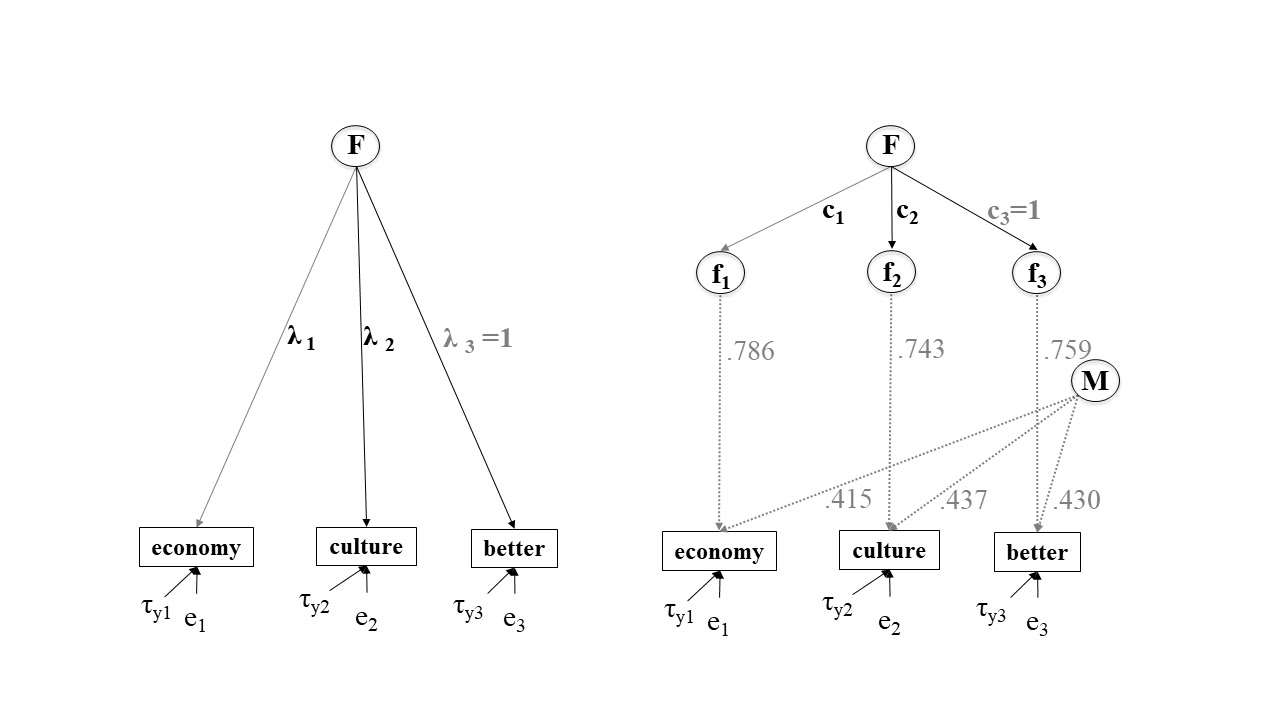
\includegraphics[width=0.8\linewidth]{correctionmodel} \caption{Measurement invariance with correction for measurement error models. Source: @Pirralha2020}\label{fig:correction}
\end{figure}

\hypertarget{sample-size-model-characteristics}{%
\subsection{Sample size \& Model Characteristics}\label{sample-size-model-characteristics}}

\begin{itemize}
\item
  Sample size cannot be too small (no rule of thumb here).
\item
  Number of items per scale is very important. Large simulation study by \citet{Pokropek2019} shows that model characteristics such as number of items per scale is at least as important as invariance testing procedure
\item
  Take into account the nature of the observed items (ordinal, continuous, nominal, dichotomous)
\end{itemize}

\hypertarget{additional-resources}{%
\section{Additional resources}\label{additional-resources}}

\begin{itemize}
\item
  Highly recommended: listen to the \href{https://quantitudethepodcast.org/listen/}{Quantitude Podcast} \href{https://www.stitcher.com/podcast/quantitude/e/66905935}{episode 12}
\item
  Measurement Invariance checklists and tutorials:

  \begin{itemize}
  \tightlist
  \item
    \href{https://www.tandfonline.com/doi/abs/10.1080/17405629.2012.686740}{van de Schoot, Lugtig \& Hox, 2012}
  \item
    \href{https://www.frontiersin.org/articles/10.3389/fpsyg.2019.01507/full}{Fischer \& Karl, 2019}
  \item
    \href{https://lavaan.ugent.be/tutorial/groups.html}{Lavaan Measurement Invariance tutorial}
  \item
    Maksim Rudnev's \href{https://maksimrudnev.com/2019/05/01/alignment-tutorial/}{Alignment Invariance testing tutorial}
  \end{itemize}
\end{itemize}

  \bibliography{book.bib,packages.bib}

\end{document}
